% Preambolo
\documentclass[12pt,a4paper]{report}

\usepackage[utf8]{inputenc}
\usepackage[T1]{fontenc}
\usepackage[english,italian]{babel}
\usepackage[norules]{frontespizio}
\usepackage{url}
\usepackage{setspace}
\usepackage{graphicx}
\usepackage{listings}
\usepackage[usenames,dvipsnames]{color}

\lstset{
	backgroundcolor=\color{white},
	breakatwhitespace=false,
	breaklines=true,
	captionpos=t,
	extendedchars=true,
	frame=single,
	keepspaces=true,
	language=C,
	numbers=left,
	rulecolor=\color{black},
	showspaces=false,
	showstringspaces=false,
	showtabs=false,
	tabsize=4,
	basicstyle=\footnotesize\ttfamily,
	keywordstyle=\bfseries\color{Green},
	commentstyle=\itshape\color{Purple},
	identifierstyle=\color{Blue},
	stringstyle=\color{Orange},
}

\newcommand{\vir}[1]{``#1''}

% Documento
\begin{document}
\doublespacing
\frenchspacing

% Frontespizio
\begin{frontespizio}
	\Istituzione{Università di Pisa}
	\Logo[6cm]{logo}
	\Dipartimento{Informatica}
	\Corso[Laurea triennale]{Informatica}
	\Annoaccademico{2013--2014}
	\Titoletto{Tesi di laurea}
	\Titolo{Implementazione di un sistema operativo \\ minimale basato su microkernel}
	\Candidato[452264]{Andrea Orrù}
	\Relatore{Antonio Cisternino}
	\Rientro{1.5cm}
\end{frontespizio}

% Abstract
\renewcommand{\abstractname}{Abstract}
\begin{abstract}
	In questa tesi presenteremo \emph{Utopia}, un sistema operativo minimale basato su \emph{microkernel}.
	Partiremo da una presentazione generale dei sistemi operativi, descrivendo le motivazioni
	alla base della loro esistenza, e le funzionalità che essi forniscono solitamente.
	Vedremo poi le varie forme in cui questo insieme di funzioni può essere realizzato.
	Infine discuteremo le scelte implementative relative al caso particolare di Utopia.
\end{abstract}

% Indice
\tableofcontents


% Introduzione
\chapter*{Introduzione}
\addcontentsline{toc}{chapter}{Introduzione}
	Il ruolo del sistema operativo (\emph{SO}) è quello di gestire le risorse hardware del calcolatore, fornendo ai programmi
	un'astrazione della macchina sulla quale vengono eseguiti. Il SO si pone dunque come intermediario fra applicazioni e
	hardware della macchina, di solito incapsulando funzioni di I/O\footnote{Input/Output}, gestione della memoria etc.
	in delle \emph{syscall}, e interrompendo liberamente (\emph{preemption}) l'esecuzione dei processi.
	
	Nel linguaggio comune si utilizza spesso la locuzione \emph{sistema operativo} comprendendo con questa definizione tutta
	una serie di applicazioni e funzionalità accessorie come l'interfaccia (grafica o testuale) e le utilità di sistema.
	Queste entità ricoprono però un altro ruolo: quello di intermediario fra gli utenti e il \vir{vero} SO.
	Per questo motivo, nel seguito si parlerà di sistema operativo solo come interfaccia tra hardware e software.\\
	
	L'esistenza dei moderni sistemi operativi è giustificata da necessità di comodità, efficienza e sicurezza.
	
	Comodità, perché la presenza di una API\footnote{Application Programming Interface} unica e coerente per comunicare con
	la grande varietà di hardware esistente libera lo sviluppatore di applicazioni dall'onere della programmazione a basso livello.
	
	Efficienza, perché alternare opportunamente l'esecuzione dei processi consente di riempire i tempi morti della CPU in cui
	i programmi attendono i risultati delle operazioni di I/O, oltre a renderne possibile l'esecuzione concorrente.
	
	Sicurezza, perché delegando la gestione della memoria al sistema operativo, ogni applicazione vive in un suo
	\emph{virtual address space}\footnote{Spazio di indirizzamento virtuale. Ogni processo vede la memoria come se fosse
	l'unico processo in esecuzione.} e non può essere influenzata da altri programmi malfunzionanti, o peggio maliziosi.\\
	
	In questa tesi è mostrato lo sviluppo di un sistema operativo multi-threading minimale ma sufficientemente evoluto
	da comprendere i \emph{driver} per le periferiche di base e consentire il porting della libreria del C e di alcune applicazioni.
	La struttura della tesi è la seguente:


% Capitoli
\chapter{Storia dei sistemi operativi}
	Nei primi calcolatori, per svolgere il proprio compito ogni programma necessitava di propri driver per le periferiche.
	Il crescente livello di complessità delle macchine e delle applicazioni ha man mano reso necessario lo sviluppo dei sistemi operativi.
	
	\section{Batch processing}
		Negli anni 50, \emph{mainframe} che occupavano intere stanze venivano programmati tramite interruttori su enormi pannelli di controllo.
		Più avanti l'introduzione delle \emph{schede perforate} permise di disaccoppiare le fasi di sviluppo
		ed esecuzione, ma soltanto un utente alla volta poteva usufruire della macchina e solo per il periodo di tempo assegnatogli.
		Il calcolatore poteva eseguire soltanto un programma per volta, fino alla sua terminazione.
		
		Questi computer erano del tutto sprovvisti di sistemi operativi. In principio il codice per il controllo della macchina doveva
		essere integrato in ciascun programma, ma a seguito dello sviluppo di \emph{assembler} e \emph{compilatori} divenne
		possibile scrivere delle librerie contenenti funzionalità standard per le operazioni di I/O.
		Questi set di funzioni possono essere considerati i primi antenati dei moderni SO.
		
		In seguito, con l'invenzione dei \emph{batch} di schede perforate, i computer divennero in grado di eseguire
		code di \emph{job} in sequenza, automatizzandone il caricamento. Parallelamente, quelle che prima erano
		solo collezioni di funzioni divennero dei \emph{monitor}, programmi avviati all'accensione della macchina e
		residenti in background. Essi si occupavano di caricare, avviare, monitorare i job e riassegnare le risorse
		hardware al termine di ciascuna esecuzione.
		
		Il primo sistema operativo ad essere utilizzato in ambienti di lavoro reali fu GM-NAA I/O, prodotto
		nel 1956 dalla divisione di ricerca della General Motors per l'IBM 704.
		
	\section{Multiprogrammazione e time sharing}
		Man mano che la potenza computazionale dei computer cresceva, diminuendo i tempi di esecuzione dei job, si faceva
		percentualmente sempre più importante la durata dei tempi morti. Anche se l'introduzione del batch processing aveva
		ridotto drasticamente i tempi di attesa fra un job e il successivo, essa non poteva far nulla per sfruttare gli intervalli
		temporali in cui il programma era in attesa delle lente periferiche di I/O, come le stampanti.
		
		Per ottimizzare l'utilizzo delle risorse fu concepito il concetto di \emph{multiprogrammazione}: diversi job
		vengono caricati sulla memoria del calcolatore; quando uno di loro raggiunge un'istruzione che richiede
		l'attesa di una periferica, lo stato del processo in esecuzione viene salvato e viene data a un altro job
		la possibilità di essere eseguito (\emph{context switch}).
		
		Un ulteriore passo avanti fu compiuto quando ci si rese conto che un singolo utente non poteva sfruttare
		appieno le risorse della macchina. Per consentire a più utenti di interagire contemporaneamente col calcolatore
		furono dunque progettati dei terminali, collegati al computer centrale, che fungevano da interfaccia.
		
		Per rendere possibile questa modalità di utilizzo, che richiede l'esecuzione virtualmente simultanea di
		più programmi, fu introdotta la tecnica del \emph{time sharing}. L'idea alla base del suo funzionamento
		è quella di assegnare brevissimi intervalli di tempo di esecuzione a ciascun processo, così che l'utente
		umano abbia l'illusione che siano eseguiti tutti contemporaneamente.
		
		La tecnica del time sharing comportava un \emph{overhead} affatto trascurabile per i calcolatori dell'epoca.
		Bisogna infatti attendere la fine del 1961 perché veda la luce CTSS\footnote{Compatible Time-Sharing System},
		il primo sistema operativo a fornirne un'implementazione funzionante.
		
		Nel 1964 l'IBM tentò per la prima volta un'opera di unificazione, sviluppando un SO per la sua serie di
		calcolatori System/360, che utilizzavano tutti lo stesso set di istruzioni e la stessa architettura di I/O.
		Fu originariamente concepito come un prodotto unico, ma a causa delle differenze fra le varie dotazioni hardware
		venne frammentato in progetti differenti: DOS/360 pensato per le macchine meno potenti, OS/360 in varie edizioni
		con e senza le funzionalità di time sharing.
		
	\section{Minicomputer e UNIX}
		A partire dalla seconda meta degli anni 60, l'uso dei transistor e delle memorie a nucleo magnetico rese
		possibile lo sviluppo di macchine molto più piccole e dai costi molto più contenuti di quelli dei mainframe.
		Esse presero il nome di \emph{minicomputer}. Alcuni dei calcolatori di maggior successo di questa categoria,
		in particolare la serie PDP, furono prodotti dalla DEC.
		
		Fu proprio su e per queste macchine, le PDP-7 prima e la PDP-11 poi, che venne sviluppato \emph{UNIX}, uno
		dei sistemi operativi più innovativi e influenti della storia, i cui principi sono ancora oggi alla base di
		molti dei più importanti OS odierni.
		
		La prima versione di UNIX vide la luce nel 1969 ad opera dei laboratori di ricerca di AT\&T e Bell, nei quali
		lavoravano tra gli altri Ken Thompson e Dennis Ritchie, ideatore del linguaggio di programmazione C.
		Le prime revisioni del sistema furono realizzate direttamente in assembly, ma nel 1972 venne operata
		una riscrittura in C che rese possibile portare UNIX su svariate altre architetture.

		Alcune delle caratteristiche più significative sono l'impiego di un filesystem gerarchico, dei file come strumenti di
		IPC\footnote{Inter-Process Communication} e la presenza di tante piccole utilità di sistema richiamabili da CLI
		\footnote{Command Line Interface} e combinabili tramite \emph{pipe}.
		L'insieme di questi concetti prende il nome di \vir{filosofia UNIX}, descritta come \vir{l'idea che la potenza di un sistema
		derivi più dalla relazione fra i programmi che da i programmi stessi} \cite{Kernighan}.
		
	\section{Home computer e interpreti BASIC}
		Intorno alla seconda metà degli anni 70, la nascita di microprocessori a 8-bit quali il MOS 6502, l'Intel 8080 e lo Zilog Z80
		incoraggiò lo sviluppo di una nuova categoria di calcolatori, dapprima appannaggio dei soli hobbisti, ma ben presto
		destinata a conquistare ampie fascie di mercato.
		
		I cosiddetti \emph{home computer}, come l'Apple II, lo ZX Spectrum o il leggendario Commodore 64, erano equipaggiati
		con quantità minimali di memoria e non possedevano le risorse hardware sufficienti per far girare efficacemente un vero
		e proprio sistema operativo. All'interno della ROM era preinstallato un interprete BASIC che fungeva da interfaccia testuale,
		e i programmi avevano il controllo totale della macchina mentre erano in esecuzione.
		
		\begin{figure}[htbp]
		\centering
		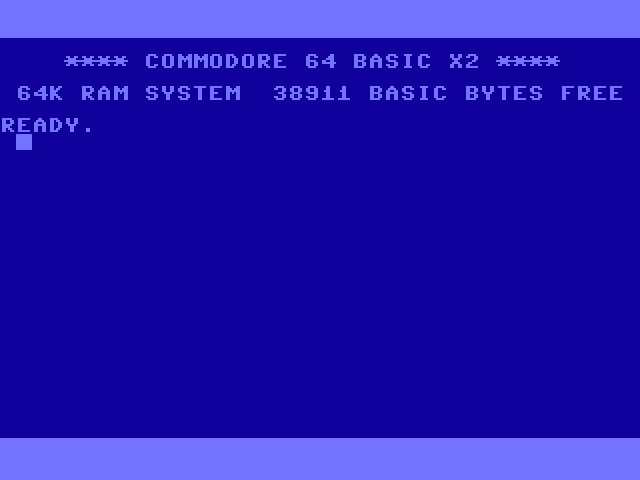
\includegraphics[scale=0.5]{img/commodore64.png}
		\caption{L'interprete BASIC del Commodore 64.\label{fig:commodore64}}
		\end{figure}
		
	\section{Personal computer}
		\subsection{IBM PC e DOS}
			Nel 1981 il colosso IBM, che dominava il settore dei mainframe ma che fino ad allora non si era occupato del mercato
			dei calcolatori domestici, introdusse l'\emph{IBM PC}, costruito attorno al processore a 16-bit Intel 8088 e con una
			architettura aperta e espandibile. Il sistema operativo scelto dall'IBM per pilotare queste macchine fu \emph{MS-DOS}, sviluppato
			dalla Microsoft sulla base di 86-DOS, del quale la società di Bill Gates aveva acquistato i diritti per 50000\$.
		
			Come la maggior parte dei sistemi operativi per home e personal computer del tempo, MS-DOS era monoutente
			e monotask \cite{WIKI_MS-DOS}. Di base forniva un'interfaccia a riga di comando con cui poter gestire i file
			e lanciare i programmi, i quali assumevano però il controllo totale del sistema una volta avviati.
			
		\subsection{Interfacce grafiche: Mac OS e Windows}
			Il primo sistema operativo a rendere popolare il concetto di GUI\footnote{Graphical User Interface} e la metafora del desktop
			fu \emph{Mac OS} \cite{WIKI_MacHistory}, il SO preinstallato sull'Apple Macintosh, lanciato nel 1984.
			La Microsoft collaborò con la Apple per la realizzazione di molte delle applicazioni del Macintosh e, a partire da questa
			esperienza, fece confluire molte delle idee dell'azienda di Cupertino nel proprio sistema operativo, Windows, la cui
			prima versione vide la luce nel 1985.
			Nelle sue prime incarnazioni, Windows non era però un SO \emph{standalone}, bensì un'estensione per MS-DOS,
			col quale condivideva l'assenza di multitasking e i limiti nella gestione della memoria.
	
			\begin{figure}[htbp]
			\centering
			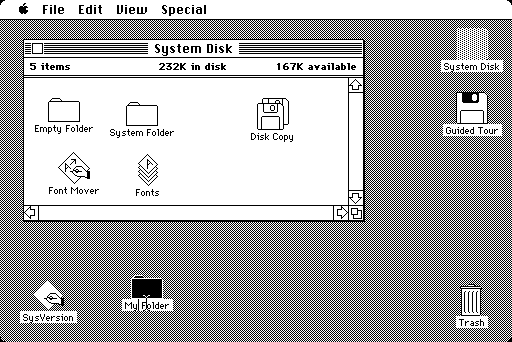
\includegraphics[scale=0.6]{img/macos.png}
			\caption{L'interfaccia grafica della prima versione di Mac OS.\label{fig:macos}}
			\end{figure}
			
		\subsection{L'Intel x86 e il multitasking su PC}
			L'introduzione da parte di Intel dei processori 386, dotati di MMU\footnote{Memory Management Unit} e quindi capaci di fornire a
			livello hardware meccanismi di protezione della memoria, aprì la strada alla realizzazione di sistemi operativi multitasking
			fino ad allora confinati ai costosi mainframe.
			...

\chapter{L'architettura x86}
	In questo capitolo daremo una descrizione sommaria dei processori Intel x86, largamente la più comune nei PC moderni.
	Porremo l'accento in particolare sulle serie a 32-bit (dalla 386 alla 686).
	
	L'obiettivo è di dare al lettore una comprensione dell'architettura sufficiente da poter apprezzare i dettagli implementativi
	illustrati nei capitoli successivi.
	
	\section{Set di istruzioni e registri}
		L'architettura x86 consiste di un set di istruzioni di lunghezza variabile, con un'impronta prevalentemente
		\emph{CISC}\footnote{Complex Instruction Set Computer} e una forte enfasi sulla retrocompatibilità \cite{WIKI_x86}.
		Questo significa che il cuore dell'instruction set è a tutt'oggi quello dei vecchi processori a 16-bit.
		
		Per illustrare questo concetto è significativo l'esempio dei registri (si veda la figura~\ref{fig:gpr}).
		Si consideri il registro AX; è possibile accedere rispettivamente ai suoi 8 bit alti e bassi tramite AH e AL.
		
		Analogamente, sui processori dal 386 in poi, aggiungendo il prefisso \textbf{E} (es. EAX) si accede al corrispondente
		registro a 32-bit, ma è ancora possibile agire sui 16 bit bassi riferendosi a AX.
		
		\begin{figure}[t]
		\centering
		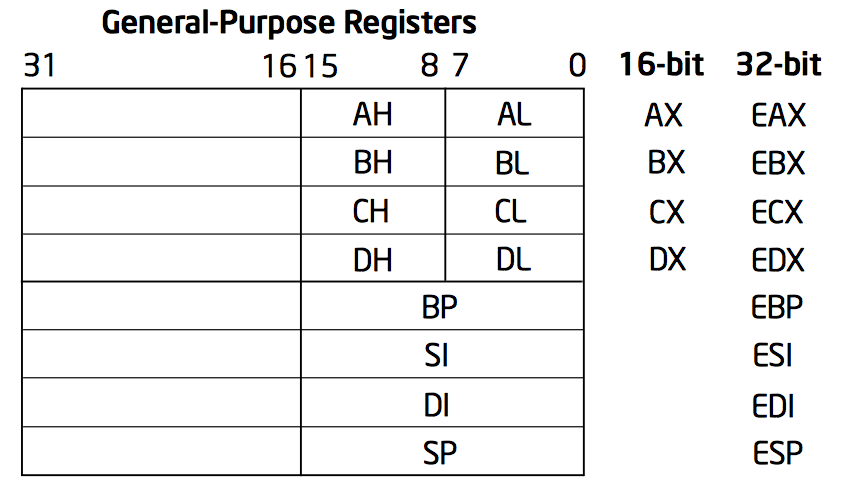
\includegraphics[scale=0.6]{img/gpr.png}
		\caption{I registri \emph{general purpose} dell'architettura x86. \cite{Intel}\label{fig:gpr}}
		\end{figure}

		\begin{figure}[b!]
		\centering
		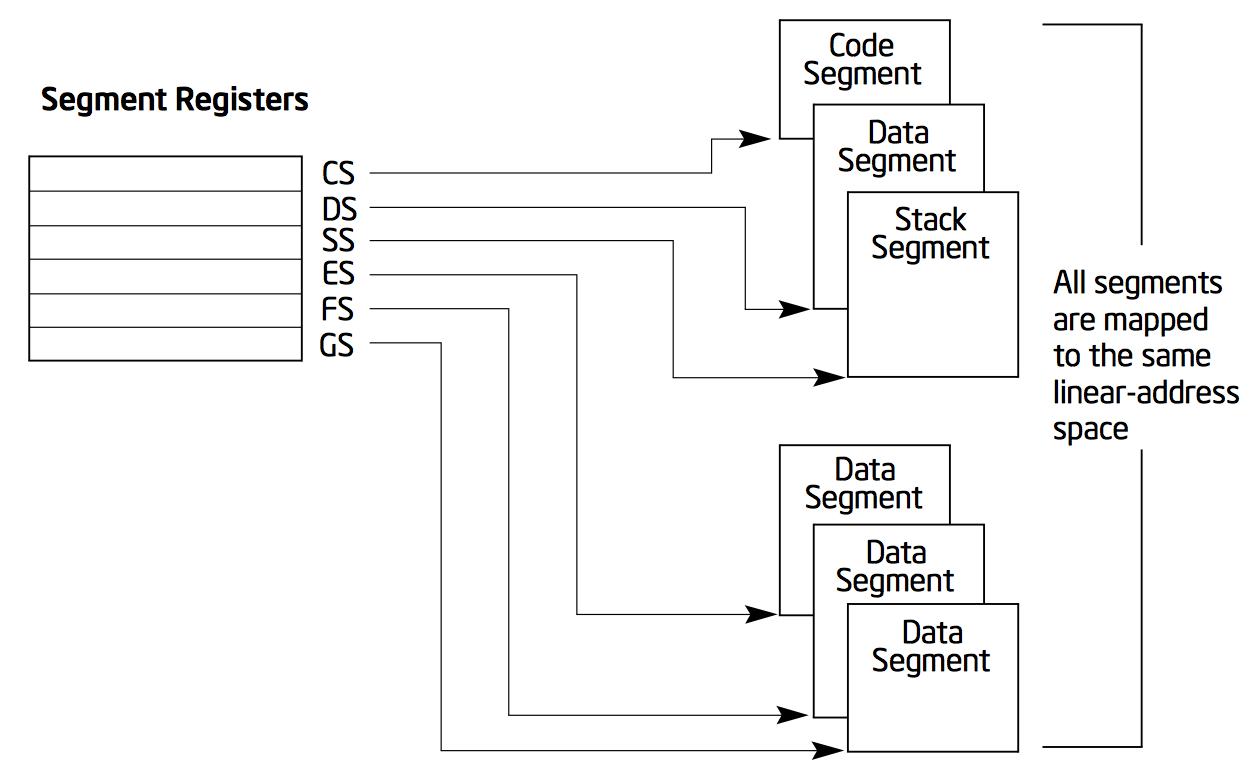
\includegraphics[scale=0.5]{img/segment.png}
		\caption{Registri segmento. \cite{Intel}\label{fig:segment}}
		\end{figure}

	\section{Modalità operative}
		\subsection{Real mode}
			Per le suddette esigenze di retrocompatibilità, tutti i processori x86 (e anche i più moderni x86-64) si avviano
			in modalità 16-bit, che in gergo prende il nome di \emph{real mode}.
			In questo assetto il processore può indirizzare solo 20 bit di memoria (1 MiB), specificati dalla somma fra
			un registro segmento (si veda la figura~\ref{fig:segment}), il cui contenuto viene shiftato di 4 bit verso sinistra,
			e un offset di 16 bit.
		
			In real mode il processore non fornisce alcun meccanismo di protezione della memoria, e il software può
			accedere direttamente alle periferiche hardware e richiamare le routine del \emph{BIOS}\footnote{Basic Input/Output System:
			un insieme di routine software memorizzato in ROM, che fornisce una serie di funzioni di base per l'accesso all'hardware del computer.}
			tramite degli \emph{interrupt software}.
		
		\subsection{Protected mode}
			Inizializzando alcune strutture dati e modificando alcuni registri di controllo si può impostare il processore
			in \emph{protected mode}. In questa modalità i registri segmento non indicano più un indirizzo assoluto,
			ma un indice in una tabella detta \emph{GDT}\footnote{Global Descriptor Table}, che consente di definire
			segmenti di 32-bit (4 GiB) e assegnare loro alcune proprietà.
			
			Fra queste, la più significativa è la possibilità di selezionare uno fra quattro \emph{protection ring} per la
			il segmento, istituendo così dei limiti sugli accessi a determinate zone di memoria.
			Diventa possibile, ad esempio, riservare un segmento di memoria al solo \emph{Ring 0} (l'anello coi privilegi più elevati),
			consentendone l'accesso solo al codice che girà in quella modalità.
			
			Tipicamente, il \emph{kernel} di un sistema operativo gira in Ring 0 (l'unica modalità che ha accesso
			a tutte le risorse del sistema), mentre le applicazioni in Ring 3 (si veda la figura~\ref{fig:ring}).
			
			\begin{figure}[htbp]
			\centering
			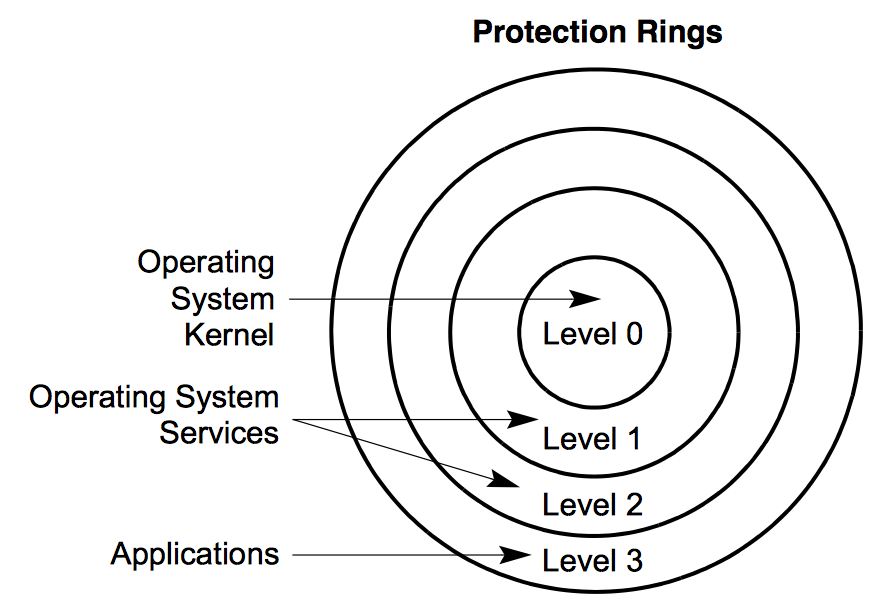
\includegraphics[scale=0.5]{img/ring.png}
			\caption{Anelli di protezione. \cite{Intel}\label{fig:ring}}
			\end{figure}
			
	\section{Paginazione}
		Una delle funzionalità più utili offerte dalla protected mode dal punto di vista dello sviluppo dei sistemi operativi
		è il \emph{paging}, un meccanismo di \emph{memoria virtuale}.
		Quando il paging è attivo, lo spazio di indirizzamento virtuale è diviso in \emph{pagine} di 4 KiB ciascuna.
		Ad ognuna di queste pagine è possibile assegnare un indirizzo di memoria fisica, riempendo delle opportune
		strutture dati interpretate dalla MMU\footnote{Memory Management Unit}, dette \emph{page tables}.
		
		\begin{figure}[htbp]
		\centering
		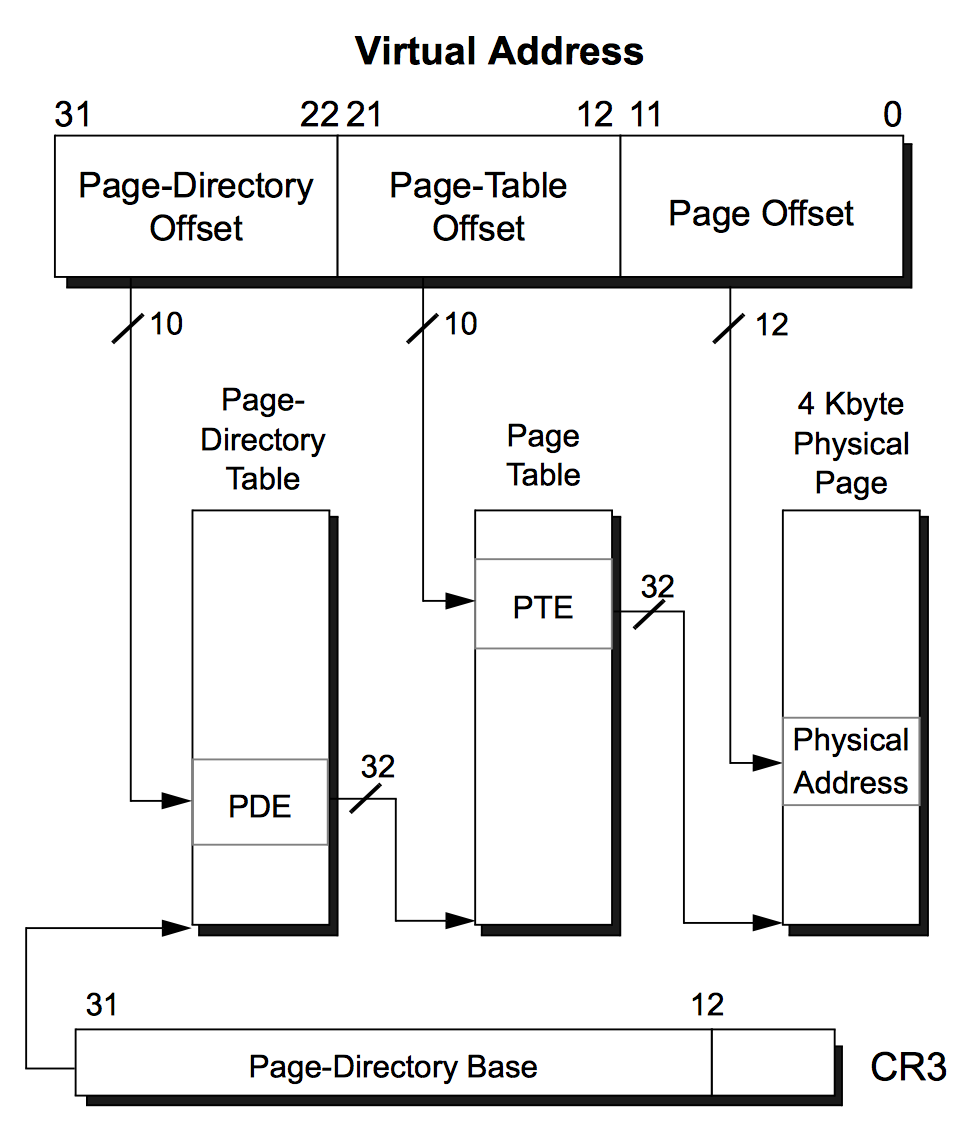
\includegraphics[scale=0.8]{img/translation.png}
		\caption{Traduzione degli indirizzi virtuali in indirizzi fisici. \cite{AMD}\label{fig:translation}}
		\end{figure}
		
		La figura~\ref{fig:translation} mostra il processo di traduzione degli indirizzi. Le page tables sono organizzate
		in due livelli.
		
		Il primo livello è quello della \emph{Page Directory}, formata da 1024 \emph{Page Directory Entry} da 4 byte
		ciascuna, per un totale di 4 KiB (la stessa dimensione di una pagina). Ognuna di queste entry, se presente, punta
		a una \emph{Page Table}, le strutture del secondo livello.
		
		Analogamente, ogni Page Table è composta da 1024 \emph{Page Table Entry} di 32 bit. Un entry, se presente,
		punta all'indirizzo della pagina fisica a cui mappare l'indirizzo di memoria virtuale corrispondente alla entry.
		
		Inserendo l'indirizzo fisico della Page Directory nel registro di controllo CR3 si comunica all'MMU il layout
		dell'address space virtuale. In un sistema operativo multitasking in cui ogni processo risiede in uno spazio
		di indirizzamento separato, il registro CR3 viene scritto ad ogni cambio di contesto fra processi.
		
		Questa operazione causa in genere l'invalidamento della cache TLB della MMU, aumentando significativamente
		il costo dei context switch.
		
	\section{Interrupt e I/O}
		\subsection{Vettori di interrupt}
			I processori x86 supportano 256 vettori di interrupt.
			I primi 32 sono riservati per le \emph{eccezioni} e sono generati dalla CPU. Divisioni per zero e \emph{page fault}
			fanno parte di questa categoria.
			
			Ci sono poi 16 IRQ, \emph{interrupt hardware} provocati dall'esterno e segnalati alla CPU dal PIC\footnote{Programmable Interrupt Controller}.
			L'IRQ 0 è generato dal timer, l'IRQ 1 dalla tastiera, e così via.
			
			Infine gli \emph{interrupt software} vengono sollevati dall'istruzione INT e sono solitamente utilizzati per richiedere l'attenzione del kernel;
			essi vengono spesso utilizzati per implementare le \emph{system call}, o chiamate di sistema \cite{OSDEV_Interrupts}.
			
			Un interrupt segnala un evento che va gestito; per fare questo viene chiamata una funzione detta \emph{Interrupt Service Routine}.
			Per permettere al kernel di definire quale funzione di gestione assegnare a ciascun interrupt esiste una tabella, detta IDT\footnote{Interrupt Descriptor Table}.
			
			Quando viene sollevato un interrupt, il processore recupera l'indirizzo dello stack del kernel, salva lo stato di alcuni registri
			nello stack (vedi figura~\ref{fig:interrupt}) e comincia a eseguire in Ring 0 il codice della funzione specificata.
						
			\begin{figure}[htbp]
			\centering
			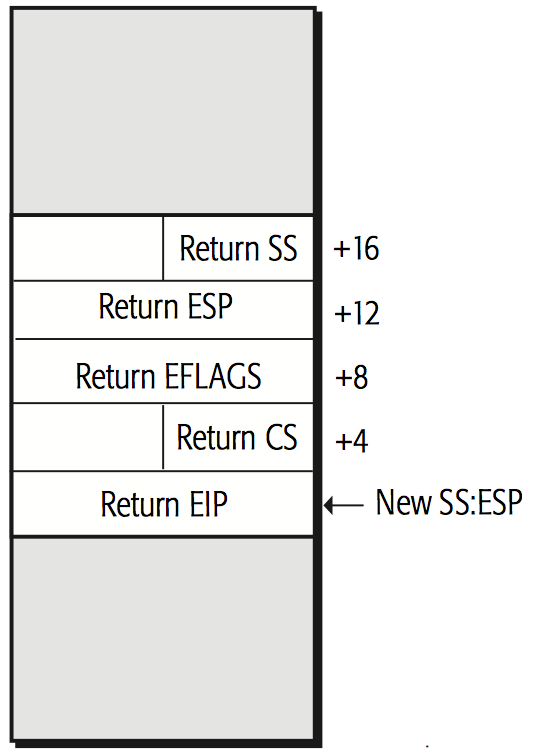
\includegraphics[scale=0.7]{img/interrupt.png}
			\caption{Lo stack dopo un interrupt avvenuto in user-mode. \cite{AMD}\label{fig:interrupt}}
			\end{figure}
			
		\subsection{I/O}
			Tramite le istruzioni IN e OUT è possibile accedere a 64 KiB di registri di I/O per comunicare con le periferiche esterne.
			Il codice eseguito in Ring 0 può accedere a tutti i registri hardware, il Ring 3 a nessuno, mentre i restanti anelli possono
			essere configurati tramite alcuni campi di una struttura dati detta TSS\footnote{Task State Segment}.
			
			Alcune entità hardware utilizzano invece il cosiddetto \emph{memory mapped I/O}: ad esempio, la VRAM della scheda
			video viene tipicamente mappata all'indirizzo 0xB8000 della memoria fisica principale.
				
\chapter{Struttura dei sistemi operativi}
	In questo capitolo forniremo una descrizione dettagliata delle componenti e dell'organizzazione di un sistema operativo e
	delle possibili soluzioni implementative. Illustreremo e metteremo poi a confronto due casi concreti, Linux e Windows.
	
	\section{Il rapporto fra hardware, kernel e applicazioni}
		\begin{figure}[htbp]
		\centering
		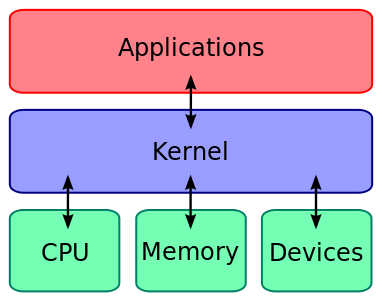
\includegraphics[scale=0.7]{img/layout.png}
		\caption{Il kernel connette le applicazioni all'hardware del computer. \cite{WIKI_Kernel}\label{fig:layout}}
		\end{figure}
		
		Come accennato nei capitoli precedenti, il sistema operativo svolge il ruolo di intermediario fra l'hardware e
		le applicazioni.
		Per fare ciò esso fornisce delle \emph{astrazioni} ad un livello più alto di quello della macchina.
		
		Ad esempio, un calcolatore può essere dotato di un certo numero di CPU, di una certa quantità
		di RAM, e di un hard disk.
		Dal punto di vista della CPU non esiste il concetto di "processo", ma solo quello di istruzioni da eseguire;
		dal punto di vista della RAM ogni zona di memoria non è assegnata ad alcuna applicazione;
		dal punto di vista dell'hard disk esistono solo settori, non file.
		
		Affinché queste astrazioni possano essere messe in atto, è necessario che il sistema operativo
		gestisca le risorse realizzando un equivalente \emph{virtuale} di ciascuna di esse.
		Il \emph{multitasking} si può pensare come la creazione di una CPU virtuale per ogni processo, emulate
		alternativamente dalla CPU fisica.
		La \emph{memoria virtuale} realizza l'illusione che ogni processo sia l'unico caricato in memoria, con
		evidenti vantaggi in termini di sicurezza.
		Il \emph{filesystem} consente di accedere a insiemi di dati eventualmente sparsi sui vari settori
		del disco semplicemente richiamandoli per nome.
		
		Come si vede, l'esistenza di queste astrazioni è funzionale a diversi obiettivi: da un lato semplifica
		il lavoro del programmatore di applicazioni fornendo interfacce coerenti e indipendenti dall'hardware,
		dall'altro incrementa la sicurezza minimizzando l'influenza che ciascun processo può avere sugli altri.
		
		Un certo insieme di queste astrazioni (almeno quelle più fondamentali) è realizzato dal \emph{kernel},
		o nucleo del sistema operativo.
		Il codice del kernel gira in \emph{stato supervisore} (Ring 0 nell'architettura x86) e ha accesso completo
		all'hardware. Tipicamente gestisce come minimo memoria fisica e virtuale, interrupt, schedulazione dei processi e
		IPC\footnote{Inter-Process Communication: comunicazione interprocesso.}. 
		I driver delle periferiche e altre astrazioni possono far parte delle responsabilità del nucleo all'interno del sistema,
		a seconda del modello di kernel scelto durante la fase di progettazione.
	
	\section{Modelli di kernel}
		\subsection{Monolitico}
			\begin{figure}[htbp]
			\centering
			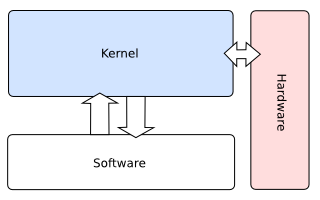
\includegraphics[scale=0.7]{img/monolithic.png}
			\caption{La struttura di un sistema a kernel monolitico. \cite{OSDEV_Monolithic}\label{fig:monolithic}}
			\end{figure}
		
			Un kernel che include tutti i driver\footnote{Programmi che gestiscono l'interazione con le periferiche hardware.} e i servizi di sistema
			nello stesso address space e con tutto il codice che gira in modalità supervisore viene detto \emph{monolitico}.
			La progettazione e l'implementazione di un kernel monolitico è generalmente ritenuta la più semplice fra i vari modelli esistenti \cite{Thompson}.
			
			In un sistema di questo tipo, qualsiasi funzione che non può essere implementata a livello di libreria fa parte
			dell'unico eseguibile del kernel \cite{WIKI_Kernel}. Di riflesso, la modalità attraverso la quale le applicazioni
			accedono a queste funzionalità è quella delle \emph{system call}\footnote{Una system call permette a un programma che
			gira in modalità utente di richiamare una funzione all'interno del kernel per eseguirla in modalità supervisore.}, o chiamate di sistema,
			solitamente presenti in gran numero nei kernel monolitici.
			
			Il principale vantaggio di questo approccio è rappresentato dall'efficienza. Dato che generalmente il kernel viene mappato
			nella memoria virtuale di tutti i processi, il costo e il numero dei cambi di contesto è decisamente ridotto. Inoltre, poiché
			tutte le componenti fanno parte dello stesso eseguibile, esse possono chiamarsi a vicenda al solo costo di una chiamata
			di funzione, senza scambi di messaggi.
			
			\subsubsection{Difetti e limitazioni}
				Per quanto semplice ed efficiente, il modello monolitico palesa alcuni evidenti difetti.
			
				Dal punto di vista dell'ingegneria del software, i kernel di questo tipo diventano spesso molto grandi in termini di
				linee di codice, il che aumenta esponenzialmente la difficoltà di mantenimento e \emph{debugging}.
			
				Oltre a questo, l'effetto dei bug non è a priori limitato a una singola componente e può avere effetti collaterali
				difficilmente prevedibili: dato che ogni funzione del kernel ha tutti i privilegi (poiché gira in modalità supervisore),
				essa può potenzialmente corrompere le strutture dati di qualsiasi altra parte, anche scorrelata.
			
				Ad esempio, anche se il cuore delle funzionalità del kernel è stabile e bug-free, un errore all'interno di un driver
				ha comunque la possibilità di far crashare il sistema.
					
		\subsection{Microkernel}
			\begin{figure}[htbp]
			\centering
			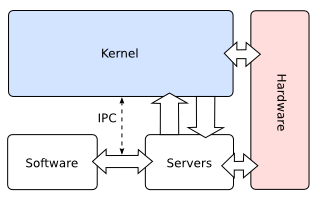
\includegraphics[scale=0.7]{img/microkernel.png}
			\caption{La struttura di un sistema a microkernel. \cite{OSDEV_Microkernel}\label{fig:microkernel}}
			\end{figure}
			
			Diversamente dal monolitico, il design del kernel a nucleo minimale (o \emph{microkernel}) cerca di
			mantenere la maggior parte del codice in user space, per cui i servizi e i driver diventano dei processi non privilegiati.
			
			Idealmente, tutto ciò per cui non è strettamente necessaria la modalità supervisore viene spostato fuori dal
			kernel. Di solito questo significa che le responsabilità del microkernel si limitano alla gestione della memoria,
			allo scheduling dei processi e all'IPC (comunicazione interprocesso). L'API\emph{Application Programming Interface}
			di un microkernel è quindi solitamente molto semplice e fornisce un numero ristretto di system call.
			
			Il grosso del sistema gira dunque su entità separate dette \emph{server} o \emph{demoni}, ognuna con un
			compito ben preciso. Dato che ogni processo risiede in un address space separato, questi programmi
			risultano ora isolati l'uno dall'altro; poiché esiste però un'interdipendenza fra le loro funzionalità, e poiché
			anche le normali applicazioni necessitano di un modo per invocarli, lo scambio di \emph{messaggi}
			tramite uno o più meccanismi di IPC forniti dal microkernel risulta cruciale.
			
			I microkernel sono composti tipicamente da poche migliaia di righe di codice, con evidenti vantaggi
			in termini di mantenibilità. A titolo di esempio, la correttezza del kernel \emph{seL4} è stata provata
			formalmente \cite{Klein}.
			Questo significa che un crash del nucleo del sistema è virtualmente impossibile. Inoltre, qualora
			fosse uno dei server a crashare, rimarrebbe sempre la possibilità di riavviarlo senza compromettere
			la stabilità del resto del sistema.
			
			\subsubsection{Difetti e limitazioni}
				Nella realtà i microkernel non sono però esenti da difetti.
				
				Un sistema a nucleo minimo è inerentemente più lento di un monolitico. Ciò che in un monolitico
				si ottiene con una semplice system call, e quindi con due soli \emph{mode switch}
				(su x86: Ring 3 => Ring 0, Ring 0 => Ring 3) e senza cambiare address space, con un microkernel
				diventa più complesso.
				
				Occorre infatti inviare un messaggio all'opportuno server tramite una delle chiamate di sistema
				per l'IPC ed effettuare un cambio di contesto, che invalida la TLB incrementando potenzialmente
				il numero di fault di cache nella MMU. Inoltre, a seconda del meccanismo utilizzato, potrebbe
				essere necessario copiare il messaggio, con ovvie ripercussioni sull'\emph{overhead} complessivo.			
				
				Infine, la già citata possibilità di riavviare le parti del sistema operativo che sono crashate è sì possibile in linea
				teorica, ma nella pratica ripristinarne lo stato può essere estremamente complicato \cite{OSDEV_Microkernel}.
	
	\section{Componenti e responsabilità del sistema}
		\subsection{Gestione della memoria}
			\subsubsection{Memoria fisica}
			\subsubsection{Memoria virtuale}
		
		\subsection{Scheduling}
			\subsubsection{Cambio di contesto}
			\subsubsection{Algoritmi di scheduling}
			
		\subsection{Comunicazione interprocesso}
			\subsubsection{Sincrona vs asincrona}
			\subsubsection{Memoria condivisa}
	
	\section{Linux}
	
	\section{Windows}

\chapter{L'implementazione di Utopia}
	Questo capitolo è dedicato alla descrizione dell'implementazione di Utopia, un sistema operativo
	minimale basato su microkernel scritto in C e Assembly x86.
	
	\section{Struttura generale e funzionalità}
		\subsection{Il microkernel}
			Il nucleo di Utopia è un classico microkernel che include soltanto le funzionalità minime per
			la gestione del sistema.
			Le motivazioni dietro questa scelta sono prettamente didattiche: si è ritenuto infatti che fosse
			più interessante, dal punto di vista delle scelte di design e dell'implementazione, realizzare
			un microkernel e alcuni server di esempio, piuttosto che un kernel monolitico.
		
			Il microkernel contiene in se la gestione degli interrupt (con notifica del loro arrivo ai processi
			che ne fanno richiesta), la gestione della memoria fisica e virtuale, un meccanismo per le chiamate
			di sistema, una forma di IPC sincrono e uno scheduler multithreading.
		
			Gli unici driver presenti all'interno del nucleo sono quello per il system timer (per ragioni
			di efficienza nello scheduling) e del terminale (per semplificare il debugging). A regime
			quest'ultimo è sostituito da un opportuno server.
			
		\subsection{I server}
			Facendo uso delle funzionalità offerte dal microkernel è possibile implementare driver
			che girano in user mode come dei processi normali. All'interno del progetto sono presenti
			il driver per la tastiera e il driver per il terminale video. Essi sono collegati rispettivamente
			a \emph{stdin} e \emph{stdout}, in maniera \emph{hardcoded} nella libreria del C.
			In versioni successive del sistema essi verranno aperti come file tramite il VFS\footnote{Virtual File System},
			un server ancora da implementare.
		
		\subsection{La toolchain GNU e la libreria C}
			Per mezzo di opportune patch ai Makefile dei software della toolchain GNU, da Binutils a GCC,
			è stato aggiunto il target \emph{i686-utopia} per poter cross-compilare software per il sistema operativo.
			
			Inoltre è stato effettuato il porting di Newlib, un'implementazione della libreria standard del C,
			che viene linkata di default alle applicazioni. Le funzioni della libreria dipendono dall'implementazione
			di un insieme di 17 syscall che devono essere fornite dal sistema. Solo alcune sono state realizzate,
			per altre è stata fornita un'implementazione \emph{dummy}.
			
			Di conseguenza la compatibilità con i sistemi POSIX non è ancora garantita.
	
	\section{Scelte progettuali e implementazione} 
		In questa sezione saranno mostrate, descritte e giustificate le parti dell'implementazione
		più significative per la comprensione del funzionamento del sistema.
	
		\subsection{La fase di caricamento}
			Nelle fasi iniziali dello sviluppo era stato scritto un \emph{bootloader} custom che caricava il kernel
			da un floppy, effettuava il salto in \emph{protected mode} e poi passava l'esecuzione al microkernel.
			
			Per ragioni di flessibilità e per la necessità di caricare moduli supplementari oltre al kernel (i server)
			si è poi optato per rendere l'eseguibile un ELF\footnote{Executable and Linkable Format} compliant con lo standard Multiboot \cite{Multiboot}.
			In questo modo il sistema può essere caricato da un bootloader come GRUB da qualsiasi tipo di supporto.
			
			Nell'header dell'eseguibile è specificato 0x100000 come indirizzo di caricamento richiesto per il kernel.
			
		\subsection{Procedura di boot del sistema}			
			Il codice nel listato~\ref{lst:main} è il primo nel microkernel vero e proprio a venire eseguito.
			La funzione riceve in input dal bootloader una struttura (descritta in \cite{Multiboot}) che contiene,
			tra le altre cose, informazioni sulle zone di memoria RAM disponibili e gli indirizzi in memoria
			degli eseguibili caricati insieme al kernel.
			
			\lstinputlisting[caption={La funzione principale del microkernel.},label={lst:main}]{code/main.c}
			
			Dalla riga 8 alla riga 14 vengono effettuate una serie di inizializzazioni sia hardware che software
			per portare il sistema a regime. Dalla linea 16 alla linea 18 vengono creati i processi corrispondenti
			ai moduli caricati dal bootloader.
			
			Infine la linea 20 abilita gli interrupt e la 21 si pone in attesa del primo \emph{tick} del \emph{system timer},
			che (come si vedrà) provoca la prima invocazione dello scheduler e l'inizio dell'esecuzione dei thread.
			
			\begin{figure}[htbp]
			\centering
			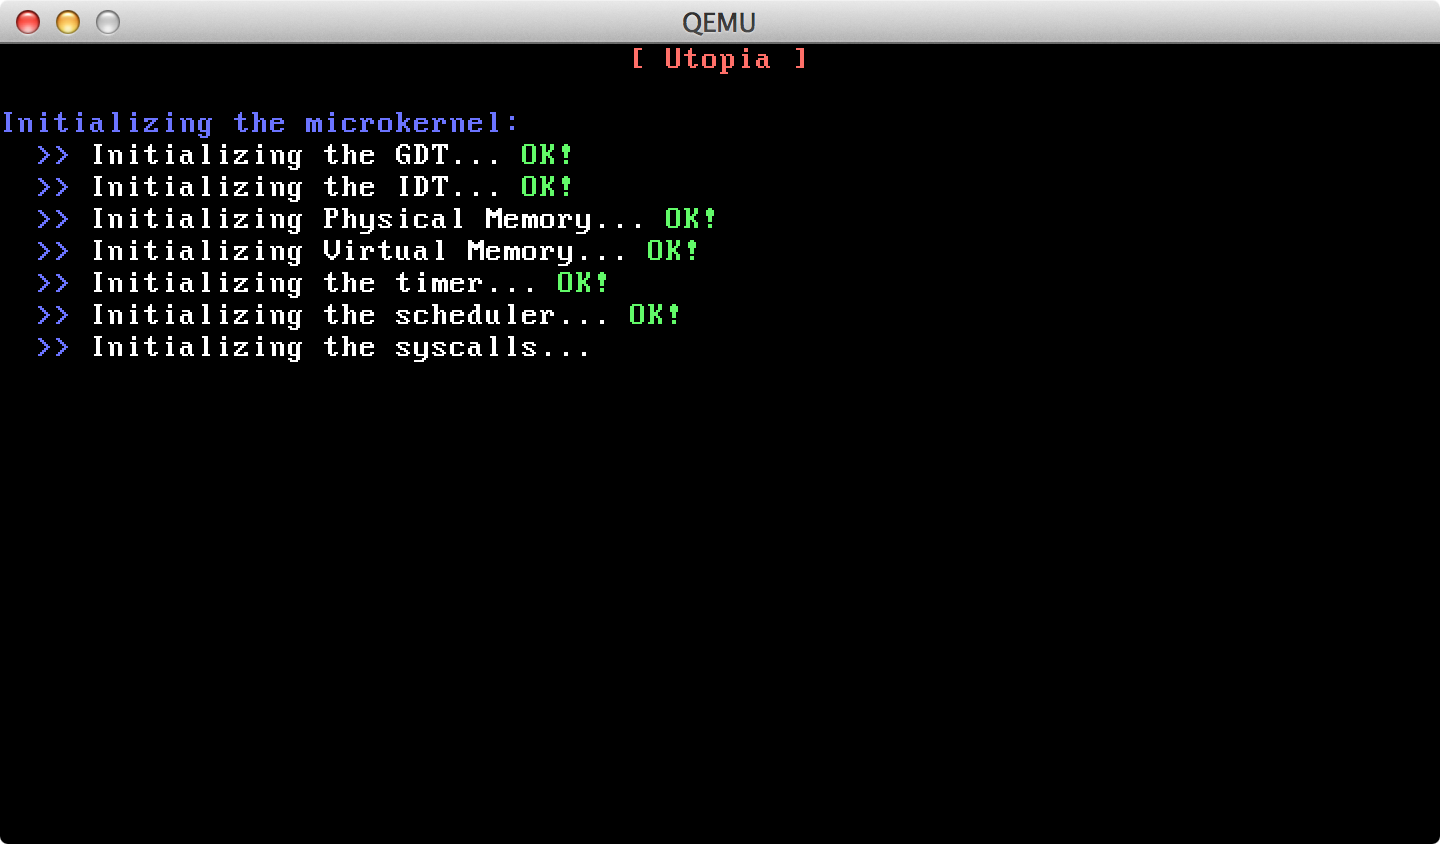
\includegraphics[scale=0.55]{img/boot.png}
			\caption{Il microkernel (in emulazione dentro QEMU) durante l'inizializzazione.\label{fig:boot}}
			\end{figure}
		
		\subsection{Gestione della memoria fisica}
			L'allocazione della memoria fisica è una delle responsabilità più basilari di un kernel.
			Per ragioni di semplicità ed efficienza si è optato per un semplice \emph{stack di frame},
			dove ogni frame è grande 4 KiB, la stessa dimensione di una pagina nell'x86, non casualmente.
			
			\lstinputlisting[caption={Il gestore della memoria fisica.},label={lst:pmem}]{code/pmem.c}
			
			La funzione pmem\_init riceve come parametro la struttura dati passata dal bootloader.
			Al suo interno è presente una mappa della memoria fisica, dove sono indicate quali
			zone di memoria sono disponibili per l'utilizzo. La mappa viene scorsa in un loop
			e ogni frame di 4KiB considerato libero viene aggiunto allo stack.
			
			Allocare o liberare un frame è a questo punto solo una questione di \emph{push} e \emph{pop} dallo stack.
			
		\subsection{Gestione della memoria virtuale}
			La gestione della memoria virtuale è una delle parti più complicate del sistema, principalmente
			a causa di una serie di caratteristiche della MMU dell'x86.
			Durante la fase di inizializzazione viene sfruttata una sua particolarità che permette,
			linkando ricorsivamente l'ultima entry della Page Directory alla Page Directory stessa,
			di mappare l'albero delle strutture del paging nell'ultimissima parte della memoria
			virtuale \cite{OSDEV_MMU}.
			In questo modo si rende più agevole la modifica del layout dell'address space corrente.
			
			\lstinputlisting[caption={La funzione che inizializza la memoria virtuale.},label={lst:vmem_init}]{code/vmem_init.c}
			
			La funzione vmem\_init inizializza il gestore della memoria virtuale.
			Alle righe 3-4 viene allocato e azzerato un frame per la Page Directory.
			
			La linea 6 mappa i primi 4 MiB di memoria fisica nei primi 4 MiB di memoria virtuale, e li imposta come \emph{globali}.
			Questa è la zona di memoria dove risiede il microkernel e le sue strutture dati; sarà mappata allo stesso modo in tutti
			gli spazi di indirizzamento, per questo si utilizza il flag PAGE\_GLOBAL, che indica alla MMU di non invalidare le voci
			corrispondenti nella TLB anche quando si cambia address space.
			
			La linea 7 effettua il mapping ricorsivo precedentemente accennato.
			Infine viene registrato il gestore dei \emph{page fault} e abilitato il paging.
			
			\lstinputlisting[caption={La funzione che mappa una pagina virtuale in una pagina fisica.},label={lst:map}]{code/map.c}
			
			La funzione map prende un indirizzo virtuale, un indirizzo fisico (o NULL) e un insieme di flag
			e mappa nell'address space corrente la pagina virtuale specificata in una fisica, con le proprietà
			indicate nei flag.
			Nel caso non venga fornito alcun indirizzo fisico, viene semplicemente allocato un frame.
			I flag specificano se la pagina è in sola lettura o anche in scrittura, se è
			riservata per lo stato supervisore o se è accessibile anche in user mode.
			
			Dalla linea 6 alla linea 12 viene verificato se la Page Directory Entry corrispondente
			all'indirizzo virtuale è già presente; in caso non lo sia, viene aggiunta e collegata ad
			un frame appena allocato e atto a contenere una Page Table, che viene poi inizializzata a zero (riga 11).
			
			Dalla linea 14 alla linea 20 viene trattato il caso in cui la pagina fisica da mappare vada allocata.
			Se la Page Table Entry è già presente (riga 16-17) si mantiene la pagina fisica corrente e si
			resettano solo i flag; in caso contrario se ne alloca una. In entrambi i casi si imposta il flag custom
			PAGE\_ALLOCATED per segnalare l'operazione.
			
			Nelle righe 21-27 viene gestito il caso in cui si sia specificata una pagina fisica particolare;
			in questo frangente, se la pagina virtuale era già mappata in un frame allocato, tale frame
			viene liberato.
			
		\subsection{Scheduling}
			L'unità di schedulazione in Utopia è rappresentata dai thread. Ogni thread all'interno di un processo
			condivide lo stesso address space, lo stesso heap ma diversi stack.
		
			\subsubsection{Processi}
				Dato che l'unità di schedulazione sono i thread, i processi fungono poco più che da contenitori.
								
				\lstinputlisting[caption={Codice per la gestione dei processi.},label={lst:process}]{code/process.c}
			
				Si analizzi la funzione process\_create. Le righe 16-17 mappano il PCB\footnote{Process Control Block}
				in una zona di memoria in \emph{kernel space} accessibile in tutti gli spazi di indirizzamento.
			
				Alla linea 20 viene creato un nuovo address space \vir{vergine} con all'interno il solo kernel space e
				il mapping ricorsivo. La riga 25 entra in questo nuovo spazio di indirizzamento e la riga 26 vi carica
				dentro l'eseguibile e crea un thread che comincerà l'esecuzione dall'\emph{entry point} del programma.
				
			\subsubsection{Thread}
				Un TCB\footnote{Thread Control Block} è grande 4 KiB, come una pagina fisica, per questioni di semplicità ed efficienza
				nell'allocazione.
			
				\lstinputlisting[caption={La struttura che descrive un thread.},label={lst:threadH}]{code/thread.h}
				
				Come si vede dal listato~\ref{lst:threadH}, la TCB è composta da due parti. La prima sezione (righe 3-16)
				contiene le varie proprietà del thread: ID globale, ID all'interno del processo, stato, informazioni sull'eventuale
				stato di attesa, processo di appartenenza.
				
				La seconda sezione (linee 17-21) è in realtà uno \emph{stack} che parte dall'estremo alto della pagina
				del TCB (si noti che nei processori x86 lo stack cresce verso il basso).
				Si è deciso di utilizzare un \emph{kernel stack} per ogni thread per motivi di semplicità ed efficienza.
				Questa scelta è piuttosto comune: il microkernel L4 adotta la stessa strategia \cite{Neider}.
				
				Ciò che accade è che al momento del passaggio da Ring 3 a Ring 0 a seguito dell'interruzione di un
				thread, il processore seleziona come stack quello inserito nel TCB, vi salva lo stato corrente (nella
				struttura Context, costruita ad-hoc) e poi esegue del codice in kernel mode continuando a utilizzare
				lo stesso stack. Terminata la gestione dell'interruzione, lo stato viene ripristinato.
				
				Si noti che avendo l'accortezza di cambiare il puntatore allo stack appena prima di ripristinare lo stato
				è possibile effettuare un cambio di contesto (si faccia riferimento al paragrafo sulla gestione delle interruzioni
				per i dettagli).
								
				\lstinputlisting[caption={Codice per la gestione dei thread.},label={lst:thread}]{code/thread.c}
				
				Il listato~\ref{lst:thread} contiene il codice per la creazione di un thread.
				Alle righe 9-10 viene mappato il TCB (che come il PCB deve essere accessibile dal kernel
				in tutti gli address space). Dalle riga 12 alla riga 20 vengono inizializzate alcune proprietà
				del thread (quelle correlate all'IPC saranno analizzate più avanti).
				
				Le linee 22-23 mappano lo stack dell'applicazione in una zona di memoria dedicata
				e diversa per ogni thread del processo.
				La linea 24 inserisce nello stack un indirizzo di ritorno speciale, che viene catturato
				dal page fault handler all'uscita del thread per garantirne la deallocazione \vir{pulita}.
				
				Le linee 26-28 allocano e mappano una pagina dedicata al TLS\footnote{Thread Local Storage},
				necessaria tra le altre cose per lo scambio di messaggi fra thread. Viene mappata sia in
				kernel space (per permettere la copia dei messaggi tra spazi di indirizzamento differenti)
				sia in user space (per permettere al thread di accedervi).
				
				Le linee 30-35 inizializzano un contesto \vir{neutro}; infine il thread viene inserito nello
				scheduler.
				
			\subsubsection{Scheduler}
				Lo scheduler usa un semplice meccanismo Round Robin: mantiene una coda di thread
				pronti e li esegue uno dopo l'altro per un certo intervallo di tempo, a meno di interruzioni
				dovute a eventi esterni (attesa di invio/ricezione, interrupt hardware, eccezioni, syscall).
				
				\lstinputlisting[caption={Le parti principali dello scheduler.},label={lst:scheduler}]{code/scheduler.c}
				
				Nella funzione scheduler\_init viene mappata globalmente una pagina il cui unico scopo è
				contenere un puntatore al TLS del thread corrente; in tal modo è esempre possibile per
				un thread in esecuzione sapere dove si trova quest'area.
				
				Inoltre viene assegnata la funzione schedule all'IRQ 0, quello del system timer; in questo modo,
				ad ogni \emph{tick} il thread in esecuzione viene bloccato e lo scheduler seleziona il successivo.
				
				La funzione schedule non fa altro che rimuovere il primo elemento dalla lista, inserirlo in fondo
				e chiamare la funzione switch_to per predisporre il cambio di contesto.
				Nel caso in cui il thread sia classificato come \emph{dying}, il suo TCB viene eliminato e si
				ripete la procedura.
				
				La funzione switch\_to esegue un cambio di address space solo se strettamente necessario,
				ovvero se si sta passando ad eseguire il thread di un processo differente da quello corrente.
				La riga 9 aggiorna il puntatore al TLS; le linee 10 e 11 aggiornano due strutture dati globali
				che contengono rispettivamente l'indirizzo del \emph{kernel stack} associato al thread (si veda
				la sezione precedente) e l'indirizzo della parte di stack dov'è conservato lo stato del thread.
				Queste informazioni saranno poi utilizzate dal gestore degli interrupt per salvare e ripristinare
				lo stato del thread.
					
		\subsection{Gestione delle interruzioni}
			Il codice delle Interrupt Service Routine (ISR) è assolutamente centrale nella struttura del sistema.
			Scheduling, cambi di contesto e chiamate di sistema fanno affidamento sul corretto funzionamento
			di queste poche ma importanti righe, scritte direttamente in assembly.
			
			Ogni ISR è una istanza della macro che segue, che prende come parametro il numero del vettore
			dell'interrupt e genera il codice per il particolare tipo di interruzione (software, hardware, syscall).
						
			\lstinputlisting[language={[x86masm]Assembler},caption={Interrupt Service Routines.},label={lst:isr}]{code/isr.asm}
			
			Alcune eccezioni hanno un codice di errore che pushano nello stack. Affinché la struttura dello stack sia la stessa
			per tutte le interruzioni, le linee 4-6 pushano un valore dummy in sostituzione del codice di errore per le interruzioni
			che non lo prevedono. La linea 7 salva il numero del vettore dell'interrupt, mentre la linea 8 salva il contenuto
			di tutti i registri \emph{general purpose}.
			
		\subsection{Comunicazione interprocesso}
		
		\subsection{Connessione fra libreria del C e sistema}

\chapter{Sviluppi futuri}


% Bibliografia
\begin{thebibliography}{}
	\bibitem{Silberschatz}
		Silberschatz A., Galvin P. B., Gagne G.,
		\emph{Operating System Concepts}.
		Wiley,
		9th Edition,
		2012.
	\bibitem{Kernighan}
		Kernighan B., Pike R.,
		\emph{The UNIX Programming Environment}.
		Prentice Hall,
		1984.
	\bibitem{Intel}
		\emph{Intel 64 and IA-32 Architectures Software Developer’s Manual}.
		Intel,
		Febbraio 2014.
	\bibitem{AMD}
		\emph{AMD64 Architecture Programmer’s Manual Volume 2: System Programming}.
		AMD,
		Maggio 2013.
	\bibitem{Klein}
		\emph{seL4: Formal Verification of an OS Kernel}.
		ACM,
		Klein G., Elphinstone K., Heiser G., e altri.
		Ottobre 2009.
	\bibitem{Neider}
		Microkernel Construction Notes.
		\emph{\url{http://i30www.ira.uka.de/~neider/edu/mkc/mkc.html}}
		Neider R.,
		Settembre 2008.
	\bibitem{Newlib}
		Newlib C library.
		\emph{\url{http://sourceware.org/newlib/}}
	\bibitem{Multiboot}
		Multiboot Specification.
		\emph{\url{http://www.gnu.org/software/grub/manual/multiboot/multiboot.html}}
	\bibitem{WIKI_OS}
		Wikipedia, Operating system.
		\emph{\url{http://en.wikipedia.org/wiki/Operating_system}}
	\bibitem{WIKI_OSHistory}
		Wikipedia, History of operating systems.
		\emph{\url{http://en.wikipedia.org/wiki/History_of_operating_systems}}
	\bibitem{WIKI_MS-DOS}
		Wikipedia, MS-DOS.
		\emph{\url{http://it.wikipedia.org/wiki/MS-DOS}}
	\bibitem{WIKI_MacHistory}
		Wikipedia, History of Mac OS.
		\emph{\url{http://en.wikipedia.org/wiki/History_of_Mac_OS}}
	\bibitem{WIKI_x86}
		Wikipedia, x86.
		\emph{\url{http://it.wikipedia.org/wiki/x86}}
	\bibitem{WIKI_Kernel}
		Wikipedia, Kernel (operating system).
		\emph{\url{http://en.wikipedia.org/wiki/Kernel_(operating_system)}}
	\bibitem{OSDEV_Monolithic}
		OSDev Wiki, Monolithic kernel.
		\emph{\url{http://wiki.osdev.org/Monolithic_Kernel}}
	\bibitem{OSDEV_Microkernel}
		OSDev Wiki, Microkernel.
		\emph{\url{http://wiki.osdev.org/Microkernel}}
	\bibitem{OSDEV_Interrupts}
		OSDev Wiki, Interrupts.
		\emph{\url{http://wiki.osdev.org/Interrupts}}
	\bibitem{OSDEV_MMU}
		OSDev Wiki, Memory Management Unit.
		\emph{\url{http://wiki.osdev.org/Memory_Management_Unit}}
\end{thebibliography}

\end{document}
